\documentclass[10pt,twocolumn,letterpaper]{article}

\usepackage{../cvpr}
\usepackage{times}
\usepackage{epsfig}
\usepackage{graphicx}
\usepackage{amsmath}
\usepackage{amssymb}

% Include other packages here, before hyperref.

% If you comment hyperref and then uncomment it, you should delete
% egpaper.aux before re-running latex.  (Or just hit 'q' on the first latex
% run, let it finish, and you should be clear).
\usepackage[pagebackref=true,breaklinks=true,letterpaper=true,colorlinks,bookmarks=false]{hyperref}

\cvprfinalcopy % *** Uncomment this line for the final submission

\def\cvprPaperID{****} % *** Enter the CVPR Paper ID here
\def\httilde{\mbox{\tt\raisebox{-.5ex}{\symbol{126}}}}

% Pages are numbered in submission mode, and unnumbered in camera-ready
\ifcvprfinal\pagestyle{empty}\fi

\begin{document}
	
	\title{Temporal Difference Variational Auto-encoder}
	\author{Karol Gregor \and George Papamakarios \and Frederic Besse \and Lars Buesing \and Théophane Weber \and DeepMind}
	\date{Jan 2019}
	
	\maketitle

	\section{Motivation}
	The authors propose that it is essential to incorporate the following characteristics in a model for dynamical systems:
	\begin{enumerate}[label=\textbf{\arabic*},ref=\arabic*]
		\item \textbf{Abstraction at the state level: } latent dynamical systems
		\item \textbf{Belief Representation: } a deterministic coding compressing the observations up to time step $t$ through \emph{LSTMs}
		\item \textbf{Jumpy State Predictions: }modeling $p(z_{t_2}|z_{t_2}), t_2>t_1 $ in the generative transitions \label{mot:jumpy}.
	\end{enumerate}
	
	\subsection{Related Works - factorization of the posterior}
	
	In many related works for modeling dynamical systems, the approximate posterior distribution $q(z_{1:T}|x_{1:T})$ is factorized autoregressively as below:
	
	\begin{equation}
	q(z_{1:T}|x_{1:T}) = \prod{q(z_t|z_{t-1}, \phi(x_{1:t}))}
	\end{equation}
	
	Using this autoregressive decomposition, one can formulate the $L_{ELBO}$ as:
	
	\begin{equation}	
	\begin{split}
	\log p(x_{1:T}) = &\E_{z \sim q(z_{1:T}|x_{1:T})} \big[\sum_{t=1}^{T} \log p(x_t|z_t) + \\ &\log p(z_t|z_{t-1}) + \log q(z_t|z_{t-1},\phi(x_{1:t}))\big] 
	\end{split} 
	\end{equation}
	
	The authors claim that this is an issue since the uncertainty of the marginal posterior of $z_t$ could be leaked in the sample $z_{t-1}$. What I believe this means is, that basing the estimation of the next state $z_t$ on one sample of the previous state $z_{t-1}$ and hoping to capture all the information about the previous observations is not enough. For an accurate posterior estimation thus, either ancestral sampling is necessary (e.g through \emph{particle filters}) or we use \emph{belief states}.
	
	\section{Problem Statement}
	
	The goal we are working towards is:
	 \begin{itemize}
	 	\item Estimating the parameters of a  State Space Model \ref{fig:SSM}
	 	\item Additionally, we want to estimate the posterior probability distribution over states $z_{1:T}$ given just the observations $x_{1:T}$ and (optional) actions $u_{1:T}$. 
	 \end{itemize}
	
	%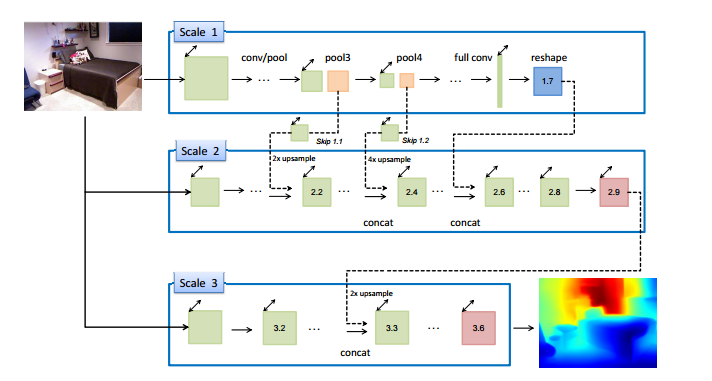
\includegraphics[width = 7.5cm, height = 4cm]{dlcv.png}
	\begin{figure}[htbp]
		\centering
		% The state vector is represented by a blue circle.
		% "minimum size" makes sure all circles have the same size
		% independently of their contents.
		\tikzstyle{state}=[circle,
		thick,
		minimum size=1.0cm,
		draw=black!80,
		fill=gray!20]
		
		% The measurement vector is represented by an orange circle.
		\tikzstyle{measurement}=[circle,
		thick,
		minimum size=1.0cm,
		draw=black!80,
		fill=purple!25]
		
		% The control input vector is represented by a purple circle.
		\tikzstyle{input}=[circle,
		thick,
		minimum size=1.0cm,
		draw=black!80,
		fill=white!20]
		
		\begin{tikzpicture}[>=latex,text height=1.5ex,text depth=0.25ex]
		% "text height" and "text depth" are required to vertically
		% align the labels with and without indices.
		
		% The various elements are conveniently placed using a matrix:
		\matrix[row sep=0.05cm,column sep=0.05cm] {
			% First line: States
			\node (z_k-2) 		 {$\cdots$};      	   &
			\node (z_k-1) [state]{$\mathbf{z}_{k-1}$}; &
			&
			\node (z_k)   [state]{$\mathbf{z}_k$};     &
			&
			\node (z_k+1) [state]{$\mathbf{z}_{k+1}$}; &
			\\
			% Second line: inputs
			\node (u_k-1) [input] {$\mathbf{u}_{k-1}$}; &
			&
			\node (u_k)   [input] {$\mathbf{u}_k$};     &
			&
			\node (u_k+1) [input] {$\mathbf{u}_{k+1}$}; &
			&
			\\
			% Third line: measurements
			&
			\node (x_k-1) [measurement] {$\mathbf{x}_{k-1}$};       &
			&
			\node (x_k)   [measurement] {$\mathbf{x}_{k}$};       &
			&
			\node (x_k+1) [measurement] {$\mathbf{x}_{k+1}$};       &
			\\
		};
		
		% The diagram elements are now connected through arrows:
		\path[->]
		(u_k-1) edge[thick] (z_k-1)
		(u_k) 	edge[thick] (z_k)	
		(u_k+1) edge[thick] (z_k+1)		
		(z_k-1) edge[thick] (x_k-1)	
		(z_k) 	edge[thick] (x_k)	
		(z_k+1) edge[thick] (x_k+1)		
		(z_k-2) edge[thick] (z_k-1)
		(z_k-1)	edge[thick] (z_k)
		(z_k)	edge[thick] (z_k+1)	
		;
		
		% Now that the diagram has been drawn, background rectangles
		% can be fitted to its elements. This requires the TikZ
		% libraries "fit" and "background".
		% Control input and measurement are labeled. These labels have
		% not been translated to English as "Measurement" instead of
		% "Messung" would not look good due to it being too long a word.
		
		% \begin{pgfonlayer}{background}
		% \node [background,
		% fit=(u_k-1) (u_k+1),
		% label=left:Entrance:] {};
		% \node [background,
		% fit=(w_k-1) (v_k-1) (A_k+1)] {};
		% \node [background,
		% fit=(z_k-1) (z_k+1),
		% label=left:Measure:] {};
		% \end{pgfonlayer}
		\end{tikzpicture}
		
		\caption{State Space Model}
		\label{fig:SSM}
	\end{figure}
	
	\section{A Lowerbound to the Autoregressive Decomposition of $p(x_{1:T})$}
	
	Instead of a lower-bound on the likelihood of the complete data sequences, the authors propose a sum of lower-bounds on the factors of an autoregressive decomposition of $p(x_{1:T})$:
	
	\begin{equation}\label{eq:autoreg_elbo_1}
	\begin{split}
	\log p(x_{1:T}) &= \sum_{t=1}^{T} \log p(x_t|x_{<t}) \\
	&\geq \sum_{t=1}^{T} \E_{z_{t-1}, z_t \sim q(z_{t-1}, z_t| x_{\leq t})} \big[\log p(x_t|z_{t-1}, z_t, x_{<t}) \\&+ \log p(z_{t-1}, z_t| x_{<t})
- \log q(z_{t-1}, z_t| x_{\leq t})\big]
	\end{split}
	\end{equation}
	
	With the markovian assumptions in place and by choosing the decomposition of the posterior as:
	
	\begin{equation}
	q(z_{t-1}, z_t| x_{\leq t}) = \underbrace{q(z_t| x_{\leq t})}_{\text{\color{red} belief}} \underbrace{q(z_{t-1}| z_t, x_{\leq t})}_{\text{\color{red} one-step smoothing}}
	\end{equation}
	
	we reformulate \ref{eq:autoreg_elbo_1} as:
	
	\begin{equation}\label{eq:autoreg_elbo_2}
	\begin{split}
	\log p(x_{1:T}) 
	&\geq \sum_{t=1}^{T} \E_{z_{t-1}, z_t \sim q(z_{t-1}, z_t| x_{\leq t})} \big[\log p(x_t|z_t) 
	\\&+ \log p(z_{t-1}| x_{\leq t-1})
+ \log p(z_t| z_{t-1}) \\&- \log q(z_t| x_{\leq t}) - \log q(z_{t-1}| z_t, x_{\leq t})\big]
	\end{split}
	\end{equation}
	
	Taking belief as $b_t = \underbrace{f_\theta(x_t, b_{t-1})}_{\color{red} \text{hidden state of an RNN}}$
	
	\begin{equation}\label{eq:autoreg_elbo_3}
	\begin{split}
	\log p(x_{1:T}) 
	&\geq \sum_{t=1}^{T} \E_{\begin{subarray}
		\centering
		z_t \sim p_B(z_t| b_{t}) \\
		z_{t-1} \sim q(z_{t-1}| z_t, b_t, b_{t-1})
		\end{subarray}} \big[\log p(x_t|z_t) 
	\\&+ \log p_B(z_{t-1}| b_{t-1})
+ \log p(z_t| z_{t-1}) \\&- \log p_B(z_t| b_{t}) - \log q(z_{t-1}| z_t, b_t, b_{t-1})\big]
	\end{split}
	\end{equation}
	
	\mytodos{Check if these equations \ref{eq:autoreg_elbo_1}, \ref{eq:autoreg_elbo_2}, \ref{eq:autoreg_elbo_3} are correct}
	
	\subsection{Jumpy version}
	As per the motivation in point \ref{mot:jumpy} in Section 1, the term wise loss is re-framed as:
	
	\begin{equation}\label{eq:jumpy_elbo}
		\begin{split}
		-\mathcal{L}_{t_1, t_2} &\geq \E_{\begin{subarray}
			\centering
			z_{t_2} \sim p_B(z_{t_2}| b_{t_2}) \\
			z_{t_1} \sim q(z_{t_1}| z_{t_2}, b_{t_1}, b_{t_1})
			\end{subarray}} \big[\log p(x_{t_2}|z_{t_2}) 
		\\&+ \log p_B(z_{t_1}| b_{t_1})
+ \log p(z_{t_2}| z_{t_1}) \\&- \log p_B(z_{t_2}| b_{t_2}) - \log q(z_{t_1}| z_{t_2}, b_{t_2}, b_{t_1})\big]
		\end{split}
	\end{equation}
	
	While it seems that the quantity $\mathcal{L}_{t_1, t_2}$ refers to $-\log p(x_t|x_{\leq t})$, this is not completely clear. \vspace{4mm}
	\par For a schematic of this architecture, see Figure \ref{fig:TDVAE_jumpy} 
	
	The total loss is written by the authors as:
	
	\begin{equation}\label{eq:total_jumpy_elbo}
	\begin{split}
	-\mathcal{L} &= \mathbb{E}_S \big[\log p(x_{t_{1:N}})\big]\\
	&\geq \mathbb{E}_S \big[\sum_{i} \E_{\begin{subarray}
		\centering
		z_{t_i} \sim p_B(z_{t_i}| b_{t_i}) \\
		z_{t_{i-1}} \sim q(z_{t_{i-1}}| z_{t_i}, b_{t_{i-1}}, b_{t_{i-1}})
		\end{subarray}} \big[\log p(x_{t_i}|z_{t_i}) 
	\\&+ \log p_B(z_{t_{i-1}}| b_{t_{i-1}})
+ \log p(z_{t_i}| z_{t_{i-1}}) \\&- \log p_B(z_{t_i}| b_{t_i}) - \log q(z_{t_{i-1}}| z_{t_i}, b_{t_i}, b_{t_{i-1}})\big]\big]
	\end{split}
	\end{equation}
	
	where $S$ is the sampling scheme for pairs.
	 
	\begin{figure*}[htbp]
		\centering
		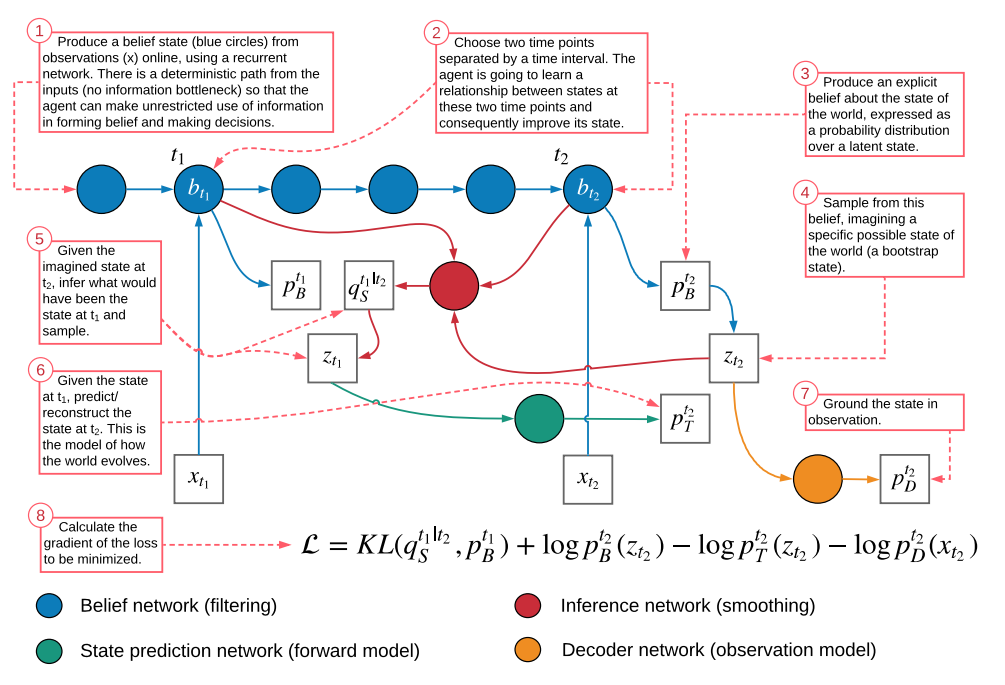
\includegraphics[width = 16cm]{TD-VAE-schematic.png}
		\caption{Schematic of TD-VAE's jumpy state model(This is from the original paper)}
		\label{fig:TDVAE_jumpy}
	\end{figure*}

\section{Discussion and Questions}
	\begin{enumerate}
		\item \textbf{Possibly incorrect decomposition of term: }\\Earlier we decomposed the quantity $p(z_{t-1}, z_t| x_{< t})$ as $p_B(z_{t-1}|b_{t-1}) \text{ and } p(z_{t-1}|z_t)$ following the chain rule decomposition and the markov assumption. The jumpy loss follows the same pattern by decomposing $p(z_{t_1}, z_{t_2}| x_{< t_2})$ as $p_B(z_{t_1}|b_{t_1}) \text{ and } p(z_{t_2}|z_{t_1})$. But in the second term of the decomposition, we cannot remove $x_{< t_2}$ from the conditional!! If we are following the graphical model in Figure \ref{fig:SSM}, the markov assumptions do not dictate that.
		\item \textbf{The possible effects of including the smoothing factor: }\\
		The authors argue that the smoothing factor $q(z_{t_1}| z_{t_2}, b_{t_2}, b_{t_1})$ is of particular significance in learning correct transitions. \vspace{4mm} \\
		They give the example of a closed box with either item A or B in it. At time $t_1$ the box is unopened, and at time $t_2$ the box has been opened and is known to have B in it. A good transition model of the box would postulate that its contents are unchanged. But sampling from just the belief at time $t_1$ wold give us item A $50\%$ of the time, which would tell us that in our transition the content of the box changes from A to B. Therefore, it's imperative to sample from the smoothing factor for the content at a previous time-step.
		\item \textbf{No sampling from the actual transition: } \\
		$z_{t_1}$ is sampled from the smoothing posterior and $z_{t_2}$ is sampled from the distribution of state given it's belief $p_B(z_{t_2}|b_{t_2})$. No parameters here are shared with the transition prior, which means the prior learns only from the KL term by the virtue of forcing the posterior to be closer to it. DVBF\cite{karl2016deep} has shown that this isn't enough to ensure that a good transition model is learned. One hypothesis about how this model works is that it relies on the smoothing factor - samples a particular future for $z_{t_2}$ from $p_B(z_{t_2}|b_{t_2})$ and makes $z_{t_1}$ stick to it .
		\item Possible \emph{non-iid} sampling when we use S, because the pairs may be related.
		\item While the images in the result section look good, they only show that the transition learns to stay within a good manifold of latent space that can give good looking reconstructions, but it doesn't show that the actual learnt transitions are good too, no results in terms of application of controls
	\end{enumerate}

	\bibliography{bib}
	\bibliographystyle{bib}
	
\end{document}